\SourcePage{GELFAND-P000449}{71}
\SourceFigure{GELFAND-P000449}{quotient-conclusion}{A short slanted stroke links $S$ to its label.
\par\smallskip\centering\color{black}
\begingroup\color{black}\GelfandFitDiagram{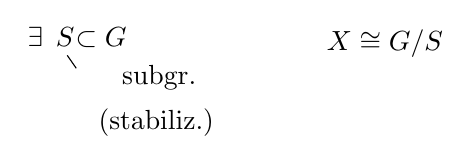
\begin{tikzpicture}[x=1mm,y=1mm,every node/.style={inner sep=0pt}]
\node[anchor=base west] (exists) at (0,13) {$\exists$};
\node[anchor=base west] (subgroup) at ([xshift=1.5mm]exists.base east) {$S$};
\node[anchor=base west] at (subgroup.base east) {$\subset G$};
\node[anchor=base west] at (38,12.6) {$X\cong G/S$};
\draw ([xshift=.25mm,yshift=-1mm]subgroup.south)--++(1.15,-1.65);
\node[anchor=base west] at (12,8.2) {subgr.};
\node[anchor=base west] at (9,2.5) {(stabiliz.)};
\end{tikzpicture}}\endgroup}
\end{GelfandAdjacentEvidence}
\begin{GelfandAdjacentEvidence}{GELFAND-P000449}{2}


\SourceFigure{GELFAND-P000449}{closing-dots}{Ten dots form a separator.
\par\smallskip\centering\color{black}
\begingroup\color{black}\GelfandFitDiagram{\begin{tikzpicture}[x=1mm,y=1mm]
\foreach \x/\y in {0/0,4/.3,9/.3,15/.4,22/.6,28/.6,33/.7,37/.5,41/.6,45/.4}
  \fill (\x,\y) circle [radius=.37mm];
\end{tikzpicture}}\endgroup}
\end{GelfandAdjacentEvidence}



\Needspace{7\baselineskip}
\begin{GelfandAdjacentEvidence}{GELFAND-P000450}{1}
